
% \documentclass[sigconf,natbib=false]{acmart}
\documentclass[sigconf,natbib=false,review,anonymous]{acmart}
%%
%% \BibTeX command to typeset BibTeX logo in the docs
\AtBeginDocument{%
  \providecommand\BibTeX{{%
    Bib\TeX}}}

%% Rights management information.  This information is sent to you
%% when you complete the rights form.  These commands have SAMPLE
%% values in them; it is your responsibility as an author to replace
%% the commands and values with those provided to you when you
%% complete the rights form.

\setcopyright{none}
\settopmatter{printacmref=false}

\copyrightyear{2027}
\acmYear{2027}
\acmConference[SAC'27]
  {The 42nd ACM/SIGAPP Symposium on Applied Computing}
  {April 5--9, 2027}
  {Gwangju, South Korea}

% DOI and ISBN are assigned after acceptance.
\acmDOI{}
\acmISBN{}


%%
%% For managing citations, it is recommended to use bibliography
%% files in BibTeX format.
%%
%% You can then either use BibTeX with the ACM-Reference-Format style,
%% or BibLaTeX with the acmnumeric or acmauthoryear sytles, that include
%% support for advanced citation of software artefact from the
%% biblatex-software package, also separately available on CTAN.
%%
%% Look at the sample-*-biblatex.tex files for templates showcasing
%% the biblatex styles.
%%
%%
%% The majority of ACM publications use numbered citations and
%% references, obtained by selecting the acmnumeric BibLaTeX style.
%% The acmauthoryear BibLaTeX style switches to the "author year" style.
%%
%% If you are preparing content for an event
%% sponsored by ACM SIGGRAPH, you must use the acmauthoryear style of
%% citations and references.

%%
%% Bibliography style
\RequirePackage[
  datamodel=acmdatamodel,
  style=acmnumeric,
  ]{biblatex}


  % ---------------------------------------------------------------------
% Packages
% ---------------------------------------------------------------------
% Packages
\usepackage{amsmath}
\usepackage{algorithm}
\usepackage{algpseudocode}
\usepackage{booktabs}
\usepackage{enumitem}
\usepackage{makecell}
\usepackage{multirow}
\usepackage{siunitx}
\usepackage{subcaption}
\usepackage{tabularx}
\usepackage{xcolor}
\usepackage{microtype}
\usepackage{tikz}
\usetikzlibrary{
    arrows.meta,
    positioning,
    fit,
    calc
}

% ---------------------------------------------------------------------
% Custom commands
% ---------------------------------------------------------------------

\newcommand{\TITLE}{\textsc{zkInfer}}
% ---------------------------------------------------------------------
% Document
% ---------------------------------------------------------------------





%% Declare bibliography sources (one \addbibresource command per source)
\addbibresource{software.bib}
\addbibresource{sample-base.bib}

%%
%% end of the preamble, start of the body of the document source.
\begin{document}

%%
%% The "title" command has an optional parameter,
%% allowing the author to define a "short title" to be used in page headers.

\title{zkInfer: Resource-Aware Distributed Proof Serving for Zero-Knowledge Machine Learning}
% Please make sure that the short title does not exceed the width of one column
% \renewcommand{\shorttitle}{Shorttitle is: Hope}

%%
%% The "author" command and its associated commands are used to define
%% the authors and their affiliations.
%% Of note is the shared affiliation of the first two authors, and the
%% "authornote" and "authornotemark" commands
%% used to denote shared contribution to the research.


%This command displays author info in page headers
% Please use the following convention:
% One author: J. Smith
% Two authors: J. Smith and I. Jones
% Three and more authors: J. Smith et al.
% \renewcommand{\shortauthors}{B. Trovato et al.}

%%
%% The abstract is a short summary of the work to be presented in the
%% article.
% ---------------------------------------------------------------------
% Abstract
% ---------------------------------------------------------------------

\providecommand{\zkTBC}[1]{\textbf{[TO COMPLETE: #1]}}

\begin{abstract}
Zero-knowledge machine learning (zkML) lets clients verify outsourced inference, but generating proofs is slow and memory intensive. Splitting a model into smaller proof jobs can reduce proving time and peak memory and allow jobs to run in parallel. However, a runtime must still decide how jobs from concurrent requests share the available compute and memory.

We characterize partitioned zkML execution and identify three properties relevant to scheduling: jobs vary widely in runtime and peak memory, a job's memory demand changes across proving stages, and repeated requests can reuse compiled circuits and proving keys. We present \emph{zkInfer}, a distributed runtime that schedules these jobs across prover nodes. A coordinator assigns jobs from active requests to nodes. Each node uses recent memory measurements to decide when a job can begin its next stage, rather than reserving its peak memory for its entire execution. zkInfer also reuses compiled circuits and proving keys without changing the underlying proving protocol.

Stage-level memory admission is most useful when available memory limits concurrency. With MobileNetV2 restricted to a 48~GiB proving budget, zkInfer reduces median request latency by 4.2--8.8\% across bursts of 2--16 requests compared with whole-job peak reservation. Separately, increasing the prover pool from one to ten nodes speeds up a single partitioned request by \(10.5\)--\(12.7\times\) across TinyBERT, MobileNetV2, and NanoGPT. Reusing setup artifacts removes 96.3--98.6\% of repeated setup time. These results show how distributed execution, stage-level memory admission, and setup reuse can improve zkML proof serving.
\end{abstract}


% ---------------------------------------------------------------------
% CCS Concepts
% Replace these with terms generated from:
% https://dl.acm.org/ccs/ccs.cfm
% ---------------------------------------------------------------------

% \begin{CCSXML}
% ...
% \end{CCSXML}

% \ccsdesc[500]{Computer systems organization~Distributed architectures}
% \ccsdesc[300]{Security and privacy~Cryptography}
% \ccsdesc[300]{Computing methodologies~Machine learning}

% ---------------------------------------------------------------------
% Keywords
% ---------------------------------------------------------------------

% \keywords{
% zero-knowledge machine learning,
% distributed proof serving,
% model partitioning,
% resource-aware scheduling,
% zero-knowledge proofs,
% machine learning inference
% }

% %%
% %% The code below is generated by the tool at http://dl.acm.org/ccs.cfm.
% %% Please copy and paste the code instead of the example below.
% %%
% \begin{CCSXML}
% <ccs2012>
%  <concept>
%   <concept_id>00000000.0000000.0000000</concept_id>
%   <concept_desc>Do Not Use This Code, Generate the Correct Terms for Your Paper</concept_desc>
%   <concept_significance>500</concept_significance>
%  </concept>
%  <concept>
%   <concept_id>00000000.00000000.00000000</concept_id>
%   <concept_desc>Do Not Use This Code, Generate the Correct Terms for Your Paper</concept_desc>
%   <concept_significance>300</concept_significance>
%  </concept>
%  <concept>
%   <concept_id>00000000.00000000.00000000</concept_id>
%   <concept_desc>Do Not Use This Code, Generate the Correct Terms for Your Paper</concept_desc>
%   <concept_significance>100</concept_significance>
%  </concept>
%  <concept>
%   <concept_id>00000000.00000000.00000000</concept_id>
%   <concept_desc>Do Not Use This Code, Generate the Correct Terms for Your Paper</concept_desc>
%   <concept_significance>100</concept_significance>
%  </concept>
% </ccs2012>
% \end{CCSXML}

% \ccsdesc[500]{Do Not Use This Code~Generate the Correct Terms for Your Paper}
% \ccsdesc[300]{Do Not Use This Code~Generate the Correct Terms for Your Paper}
% \ccsdesc{Do Not Use This Code~Generate the Correct Terms for Your Paper}
% \ccsdesc[100]{Do Not Use This Code~Generate the Correct Terms for Your Paper}

% %%
% %% Keywords. The author(s) should pick words that accurately describe
% %% the work being presented. Separate the keywords with commas.
% \keywords{Do, Not, Us, This, Code, Put, the, Correct, Terms, for,
%   Your, Paper}


%%
%% This command processes the author and affiliation and title
%% information and builds the first part of the formatted document.
\maketitle

% ---------------------------------------------------------------------
% Main sections
% ---------------------------------------------------------------------




\section{Introduction}

\label{sec:intro}

Machine-learning inference is increasingly outsourced to remote services, as modern models often require more computation, memory, and specialized hardware than clients can practically provision locally~\cite{zhang2024hardware,sheng2023flexgen}. In this setting, the service provider controls model execution, while the client typically observes only the returned prediction. The client therefore has no direct assurance that the specified model was evaluated correctly on the submitted input~\cite{kang2024scaling,qu2025zkgpt}. Verifying the result by independently re-executing the model would undermine the efficiency gains of outsourcing~\cite{kang2024scaling}, while inspecting the provider's execution may require access to proprietary model parameters, intermediate values, or other information that either party wishes to keep confidential. 


Zero-knowledge machine learning (zkML) addresses this problem by allowing the service provider to return a cryptographic proof alongside the prediction  ~\cite{chen2024zkml,kang2024scaling,boyuan2021zen,chen2025zktorch}. The proof attests that the specified model computation was executed correctly, while the client verifies the result without repeating the inference. Depending on how the computation is encoded, sensitive values such as model parameters and client inputs can remain hidden from the verifier. 

Many zkML systems~\cite{chen2024zkml,boyuan2021zen} build on zero-knowledge succinct non-interactive arguments of knowledge (ZK-SNARKs)~\cite{bitansky2012extractable,groth2016size}. ZK-SNARKs provide compact proofs with low verification cost, allowing clients to efficiently validate inference results. Their non-interactive form also allows proofs to be stored and verified later by the client or an independent auditor, without further interaction with the prover. The resulting asymmetry is attractive for verification, but places most of the computational burden on the prover.
To prove an inference, the model computation is encoded as arithmetic constraints in a proving framework such as Halo2~\cite{halo2}. For each inference, the prover constructs a witness containing the private inputs and intermediate values needed to satisfy these constraints, and then executes the proving protocol over that witness. This process can be orders of magnitude slower than ordinary inference and can consume large amounts of memory. For example, zkGPT~\cite{qu2025zkgpt} reports 147.7 seconds to prove the generation of 64 tokens, compared with 94.55 milliseconds for the corresponding model execution on the same machine, with peak prover memory reaching 240.5~GB. 


Furthermore, scalability is limited not only by the cost of generating an individual proof, but also by how proving work is scheduled across concurrent inference requests. Existing zkML systems primarily improve the efficiency and practicality of individual proofs through zk-friendly model transformations and optimized circuit construction~\cite{boyuan2021zen,chen2024zkml}, broader model support through frameworks such as EZKL~\cite{ezkl}, and increasingly through GPU acceleration~\cite{sin2024zkllm}, parallel proof accumulation~\cite{chen2025zktorch}, or decomposition into independently provable partitions~\cite{sanjaya2026zkcomposer}. These techniques reduce prover overhead and expose greater parallelism within individual proofs, but largely leave open the complementary serving problem of coordinating many independent inference requests that contend for finite prover memory and compute resources.


As zkML systems move beyond one-off proof generation, they are likely to face the same basic operating condition as conventional inference services, where requests arrive over time and compete for a finite pool of compute and memory. Unlike ordinary inference, however, each request may expand into multiple heterogeneous proof jobs whose resource demands change across proof-construction stages, making concurrent execution a central systems problem.  
Our characterization in Section\ref{sec:characterization}, across three model families, highlights these challenges. Model partitioning exposes parallel proof jobs and can reduce end-to-end proving time, but the resulting jobs vary substantially in execution time and peak memory demand. Resource usage also changes over the course of proof construction, with later cryptographic stages capable of imposing much higher memory demands than earlier preparation stages. Repeated executions of the same circuit can further reuse expensive setup state, making placement sensitive to where that state is already available.  
Together, these properties make naive concurrency ineffective. Launching
too many jobs can oversubscribe memory and cause failures, while reserving
each job's peak demand for its entire lifetime can leave substantial
capacity idle. A zkML serving runtime must therefore decide both
\emph{where} proof jobs execute and \emph{when} resource-intensive
stages may proceed, while accounting for contention and reusable setup
artifacts.

\textbf{Our Work.}
To address this gap, we introduce \TITLE{}, a distributed proof-serving system for zkML inference under concurrent workloads. \TITLE{} partitions the model's computational graph into separately provable components, turning each inference request into a collection of smaller proof jobs. Before proof generation, it computes the intermediate tensor values required at partition boundaries, allowing the resulting jobs to execute independently across prover machines. Cryptographic commitments bind the inputs and outputs of adjacent partitions so that their proofs collectively establish a consistent end-to-end inference. This decomposition exposes parallelism within each request while also creating proof jobs that can be scheduled across concurrent requests.

To coordinate proof execution, \TITLE{} uses a hierarchical resource-management architecture. A global coordinator assigns each proof job to a prover node, while a local scheduler on that node decides when the job's execution stages can run. Instead of fixing the number of concurrent workers or reserving each job's peak memory for its full lifetime, the local scheduler uses resource profiles from prior executions of the same circuit together with the node's current capacity to admit work dynamically. This allows stages from different requests to overlap when their
high-demand phases do not coincide, while keeping each proof job on a
single node throughout execution and avoiding mid-execution migration.



\TITLE{} also exploits the repeated structure of ML inference. Compiled circuits, proving keys, and other setup artifacts can be reused across executions of the same circuit. Because these artifacts are expensive to generate and may also be costly to transfer between machines, the global coordinator considers both resource feasibility and whether the required state is already present on a candidate node. Previously unseen circuits can still execute from a cold start, while recurring workloads benefit from cached proving state and resource profiles learned from prior executions.Compiled circuits, proving keys, and other setup artifacts can be reused

We implement \TITLE{} as a proof-serving layer around existing zkML
backends, with EZKL~\cite{ezkl} as the primary backend and Halo2~\cite{halo2} as the
underlying proof system. The prototype includes the global coordinator,
node-local resource managers, isolated prover processes, and reusable
artifact storage, while leaving the underlying proving protocol
unchanged. We additionally instrument EZKL and Halo2 to expose execution
stages and resource usage for characterization and online admission
decisions.

We evaluate \TITLE{} across convolutional, generative, and transformer
workloads, first isolating the effect of decomposition and then measuring
parallel, distributed, and concurrent execution. On a single worker,
partitioned execution reduces end-to-end proving latency by up to
\(5.6\times\) relative to monolithic proving. Distributing the resulting
proof jobs across multiple prover nodes further reduces latency by up to
\(69\times\) and lowers peak per-machine memory by up to \(48\times\).
\textbf{[Add concurrent-serving result here once finalized.]}

Taken together, these results show that decomposition alone does not
resolve the systems challenges of scalable zkML proving. Once an
inference is expressed as a collection of independently executable proof
jobs, the runtime must manage differences in job cost, changing resource
demand, reusable proving state, and contention across concurrent
requests. \TITLE{} addresses these concerns jointly by treating
partitioned proof generation as a distributed serving problem rather than
only as a source of parallelism within an individual inference.

\textbf{Contributions.} This paper makes the following contributions:

\begin{itemize}
   \item We characterize partitioned zkML inference as a proof-serving
workload. Across convolutional, generative, and transformer models,
we show that proof jobs differ substantially in runtime and memory
demand, that resource usage changes over the lifetime of a job, and
that repeated executions exhibit predictable resource behavior while
allowing expensive setup artifacts to be reused.

    \item We design and implement \TITLE{}, a distributed proof-serving
    runtime for concurrent zkML inference. \TITLE{} separates
    cluster-wide job placement from node-local resource admission,
    using historical execution profiles, current machine capacity, and
    reusable proving state to decide where proof jobs should run and when
    resource-intensive stages may proceed.

    \item We evaluate \TITLE{} across multiple model families and
    deployment scales. Partitioned execution reduces end-to-end proving
    latency by up to \(5.6\times\) on a single worker, while distributed
    execution achieves up to \(69\times\) lower latency than monolithic
    proving and reduces peak per-machine memory by up to \(48\times\).
    \textbf{[Add final concurrent-serving result here once available.]}
\end{itemize}






\section{Background}
\label{sec:background}

\subsection{zkML Workflow and Proving Pipeline}
\label{sec:zkml-pipeline}

As shown in Figure~\ref{fig:zkml-workflow}, a client submits an input \(x\) to a model provider, which evaluates a model with parameters \(\theta\) to produce \(y=f(x,\theta)\). The provider returns \(y\) together with a ZK-SNARK proof \(\pi\) attesting that the specified computation produced that output. Which values are public or private depends on the application.

To generate \(\pi\), the model is mapped to a proof-compatible representation, often using quantized integer or fixed-point arithmetic~\cite{boyuan2021zen,chen2024zkml}, and compiled into an arithmetic circuit or constraint system~\cite{gabizon2019plonk}. Circuit-specific proving and verification keys can be prepared ahead of time or generated on demand and reused across requests that share the same circuit configuration. For each request, the prover constructs the \emph{witness}, containing the private values required to satisfy the circuit constraints, and generates \(\pi\). The client verifies the proof using the verification key without re-executing the inference.

\begin{figure}[t]
    \centering
    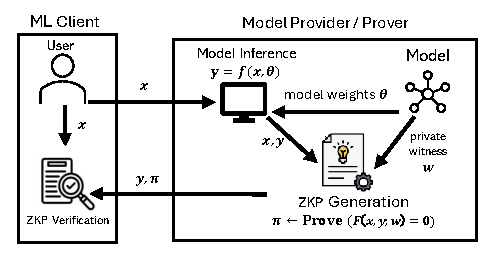
\includegraphics[width=\linewidth]{figures/background/zkInfer_workflow.pdf}
    \caption{zkML inference and verification workflow. The model provider returns an output $y$ and a proof $\pi$ attesting that $y$ was produced by evaluating the claimed model on input $x$.}
    \Description{Diagram showing a client sending an input to a machine-learning service provider. The provider evaluates a model, generates a zero-knowledge proof of correct inference, and returns the output and proof to the client, which verifies the proof.}
    \label{fig:zkml-workflow}
\end{figure}

\subsection{Proof Generation as a Systems Bottleneck}
\label{sec:proving-bottleneck}

zkML proving is substantially more expensive than ordinary model execution because the prover must demonstrate that an arithmetic constraint system is satisfied. Operations such as fixed-point arithmetic, nonlinearities, comparisons, and range checks may introduce additional constraints or lookup arguments~\cite{chen2024zkml,kang2024scaling,liu2021zkcnn}. Proof generation also materializes witness, circuit, proving-key, and polynomial data that can make the working set much larger than the model's inference activations.

These costs create systems-level constraints. Long proof times increase request latency, while large working sets restrict both the size of proof jobs that can execute on a machine and the number that can overlap safely. The problem becomes more pronounced in a serving setting, where multiple inference requests compete for finite compute and memory.

\begin{figure}[t]
\centering
\scriptsize
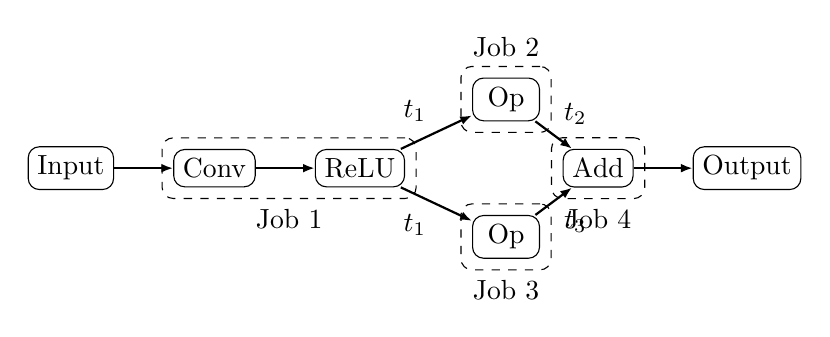
\begin{tikzpicture}[
op/.style={draw, rounded corners, minimum width=0.85cm, minimum height=0.42cm, align=center},
job/.style={draw, dashed, rounded corners, inner sep=4pt},
edge/.style={-{Latex[length=1.5mm]}, thick},
node distance=0.55cm and 0.75cm
]
\node[op] (x) {Input};
\node[op, right=of x] (conv) {Conv};
\node[op, right=of conv] (relu) {ReLU};
\node[op, above right=0.35cm and 0.85cm of relu] (a) {Op};
\node[op, below right=0.35cm and 0.85cm of relu] (b) {Op};
\node[op, right=2.0cm of relu] (add) {Add};
\node[op, right=of add] (y) {Output};
\draw[edge] (x) -- (conv);
\draw[edge] (conv) -- (relu);
\draw[edge] (relu) -- node[above left] {$t_1$} (a);
\draw[edge] (relu) -- node[below left] {$t_1$} (b);
\draw[edge] (a) -- node[above right] {$t_2$} (add);
\draw[edge] (b) -- node[below right] {$t_3$} (add);
\draw[edge] (add) -- (y);
\node[job, fit=(conv)(relu), label=below:{Job 1}] {};
\node[job, fit=(a), label=above:{Job 2}] {};
\node[job, fit=(b), label=below:{Job 3}] {};
\node[job, fit=(add), label=below:{Job 4}] {};
\end{tikzpicture}
\caption{Example inference graph partitioned into four proof jobs. Intermediate tensors \(t_1\), \(t_2\), and \(t_3\) cross job boundaries and define the interfaces between jobs.}
\label{fig:prover-job-graph}
\end{figure}

\subsection{Model Computation as a Graph}
\label{sec:model-graph}

Many zkML pipelines represent a model as an ONNX computation graph whose nodes are tensor operators and whose edges carry intermediate tensors~\cite{onnx-paper}. Figure~\ref{fig:prover-job-graph} shows how this graph can be partitioned into proof jobs. Each job contains one or more operators and proves the corresponding portion of the computation. When an edge crosses a partition boundary, the upstream tensor becomes an input to the downstream job. Partitioning therefore determines both the computation assigned to each proof job and the intermediate values that connect jobs, providing a natural structure for independently schedulable proof work.

\providecommand{\zkTBC}[1]{\textbf{[TO COMPLETE: #1]}}

\section{Characterizing zkML Serving Workloads}
\label{sec:characterization}

We characterize the properties of partitioned zkML workloads that shape
scheduling in a shared prover. We focus on three questions: how partitioning
changes proving cost, how runtime and memory vary across proof jobs, and how
memory demand evolves within a job.

\subsection{Workloads and Measurement Method}
\label{sec:characterization-method}

We use TinyBERT, MobileNetV2, and NanoGPT (4L), spanning convolutional,
encoder, and autoregressive models. At the finest granularity they produce
120, 100, and 181 proof jobs, respectively. We compare monolithic proving
with partitioned proving in which all jobs execute sequentially on the same
prover, isolating the effect of proving granularity from inter-job parallelism.
Both use EZKL~\cite{ezkl} on a dual-socket AMD EPYC 9354 server with
755~GiB of RAM. We record per-job execution time, process memory, and major
proof-stage transitions. Unless otherwise stated, runs begin cold so that the
full setup and proving lifecycle is represented.

\subsection{Impact of Partitioning on Proving Cost}
\label{sec:decomposition-benefit}

Figure~\ref{fig:partition-benefits} shows that partitioning reduces proving
time even when jobs execute serially. Relative to monolithic proving,
completion time falls by 40.6\% for TinyBERT, 16.3\% for MobileNetV2, and
60.5\% for NanoGPT (4L). Peak memory falls by 80.5\%, 91.5\%, and 98.0\%,
respectively. Partitioning also makes larger models feasible: monolithic
NanoGPT (10L) exhausts available memory, whereas partitioned execution
completes with a 12.0~GiB peak.

\textbf{Implication.}
Partitioning changes the workload presented to the runtime by reducing the
cost and memory footprint of individual proof jobs while exposing additional
parallelism.

\begin{figure}[t]
    \centering
    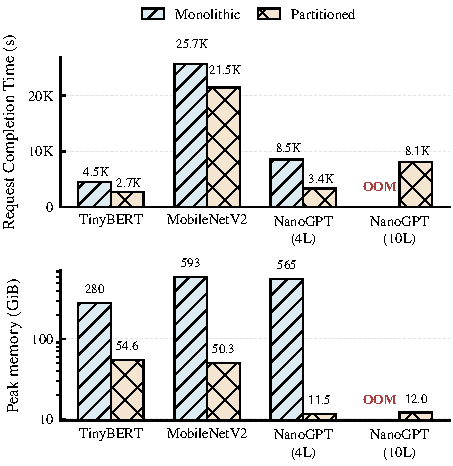
\includegraphics[width=\columnwidth]{figures/sacdad/partitioning_benefits.pdf}
    \caption{Monolithic and partitioned proving. Partitioned request time is
    the sum of proof-job runtimes; memory is the largest observed job footprint.
    OOM indicates that proving exceeded available memory.}
    \label{fig:partition-benefits}
\end{figure}

\begin{figure*}[t]
    \centering
    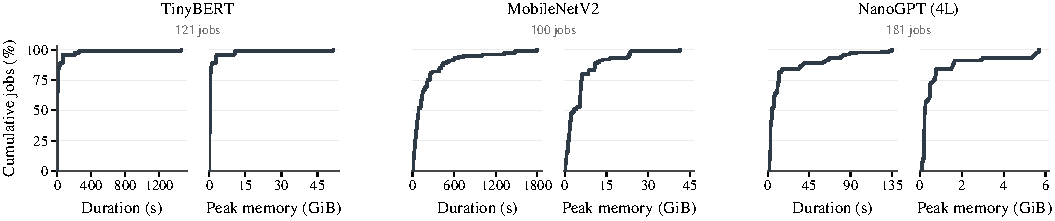
\includegraphics[width=\textwidth]{figures/sacdad/job_heterogeneity.pdf}
    \caption{Empirical distributions of proof-job execution time and peak
    memory for TinyBERT, MobileNetV2, and NanoGPT (4L).}
    \label{fig:job-heterogeneity}
\end{figure*}

\subsection{Heterogeneity Across Proof Jobs}
\label{sec:job-heterogeneity}

Figure~\ref{fig:job-heterogeneity} shows substantial heterogeneity within
each request. TinyBERT's longest job takes 1,461.3~s compared with a 4.47~s
median, a \(327\times\) difference, and accounts for 40.9\% of aggregate
job time. MobileNetV2 and NanoGPT show smaller but still substantial spreads
of approximately \(21\times\) and \(31\times\).

Memory is similarly uneven. Median per-job peaks are 0.21, 3.38, and
0.22~GiB for TinyBERT, MobileNetV2, and NanoGPT, while the largest reach
51.61, 41.45, and 5.70~GiB. A fixed concurrency limit therefore says little
about either remaining request work or instantaneous memory pressure.

\textbf{Implication.}
Runtime estimates help identify jobs that may dominate request completion,
while memory estimates determine which jobs can safely share a prover node.

\begin{figure*}[t]
    \centering
    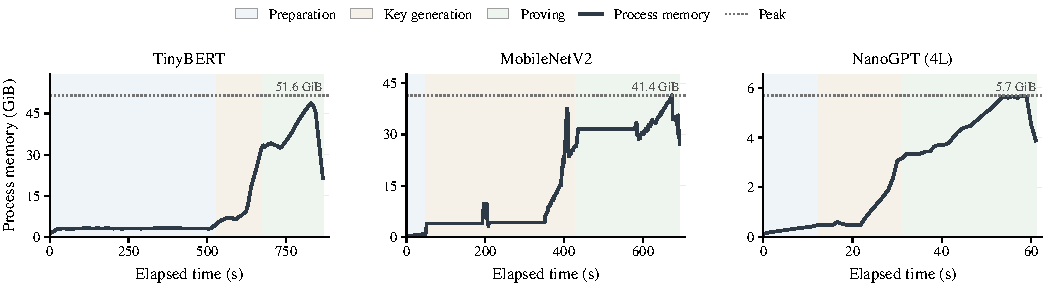
\includegraphics[width=\textwidth]{figures/sacdad/stage_memory.pdf}
    \caption{Memory demand over time for the highest-memory proof job in each
    workload. Shaded regions identify preparation, key generation, and proving.}
    \label{fig:stage-memory}
\end{figure*}

\begin{table}[t]
\centering
\setlength{\tabcolsep}{5pt}
\renewcommand{\arraystretch}{1.1}
\begin{tabular}{lcc}
\toprule
Workload & \shortstack{Time at $\geq90\%$\\of peak (\%)} &
\shortstack{Peak / average\\memory} \\
\midrule
TinyBERT      & 4.8  & $4.07\times$ \\
MobileNetV2   & 3.5  & $2.53\times$ \\
NanoGPT (4L)  & 13.3 & $2.22\times$ \\
\bottomrule
\end{tabular}
\caption{Temporal variation in memory demand for the highest-memory job in
 each workload.}
\label{tab:temporal-memory}
\end{table}

\subsection{Resource Demand Across Execution Stages}
\label{sec:stage-resource-demand}

Peak memory does not reveal how demand evolves during execution. We therefore
align process-memory samples with preparation, key generation, and proving.
Figure~\ref{fig:stage-memory} shows that the highest-memory jobs spend only
4.8\%, 3.5\%, and 13.3\% of execution at or above 90\% of peak memory for
TinyBERT, MobileNetV2, and NanoGPT, respectively. Their peaks are
\(4.07\times\), \(2.53\times\), and \(2.22\times\) their time-averaged
memory consumption (Table~\ref{tab:temporal-memory}).

\textbf{Implication.}
Whole-job peak reservation is conservative for much of execution. A runtime
can expose additional concurrency by admitting stages according to their
current memory demand rather than reserving every job's eventual peak for its
entire lifetime.

\begin{figure*}[t]
    \centering
    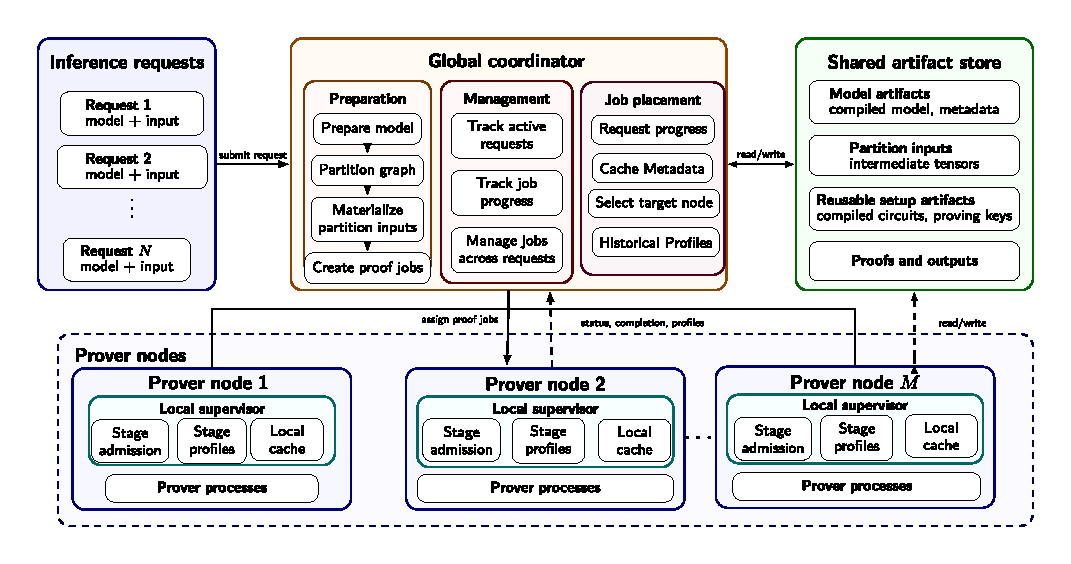
\includegraphics[width=\textwidth]{figures/sacdad/architecture.pdf}
    \caption{Architecture of \TITLE{}. A global coordinator places proof jobs
    across prover nodes, while each node performs local stage admission using
    current memory availability and historical resource profiles.}
    \label{fig:architecture}
\end{figure*}

\section{zkInfer Design}
\label{sec:design}

\subsection{System Overview}
\label{sec:system-overview}

Building on Section~\ref{sec:characterization}, we design \TITLE{} as a
distributed runtime for serving zkML proofs under concurrent requests. A
request consists of a model and inference input. \TITLE{} applies the
configured partitioning policy, materializes the corresponding
per-partition inputs, and creates proof jobs that can execute across a pool
of prover nodes. The underlying proving protocol and proof-composition
mechanism remain unchanged.

Figure~\ref{fig:architecture} shows the architecture. The coordinator
maintains jobs from all active requests and assigns whole jobs to prover
nodes. Each node then controls when the assigned job's proving stages may
run. This separation is central to the design: the coordinator handles
request-level fairness, coarse placement, and setup locality, while the
node supervisor uses current local memory and stage-level estimates for
fine-grained admission.

\subsection{Partitioning and Self-Contained Proof Jobs}
\label{sec:self-contained-proving-jobs}

During request preparation, \TITLE{} partitions the model graph according
to a system-wide policy. Unless otherwise stated, we use one graph operator
per proof job. Section~\ref{sec:eval-sensitivity} evaluates coarser
partitions.

A partition may consume tensors produced elsewhere in the graph. \TITLE{}
therefore executes the model once before distributed proving to materialize
values that cross partition boundaries and attaches them to the consuming
jobs as witness inputs. Each job can then be scheduled independently of the
execution order of other jobs. Correctness does not rely on trusting these
values directly. Each partition is proved separately, while the backend's
existing proof-composition mechanism binds values produced by upstream
partitions to those consumed downstream~\cite{ezkl-splitting}.

\subsection{Cluster-Wide Job Placement}
\label{sec:global-placement}

The coordinator first chooses a request using round-robin fairness, then
selects a job from that request. Requests with no eligible job for the
polling node are skipped for that poll, and a request moves to the back of
the queue after an assignment if work remains. This prevents a large
request from monopolizing newly available prover capacity without requiring
preemption.

Let \(\widehat{m}^{\max}_j\) and \(\widehat{d}_j\) denote the predicted
maximum memory demand and duration of job \(j\). A job is ineligible for a
node if its known peak exceeds that node's physical memory. The coordinator
does not require the whole-job peak to fit within currently free memory,
because later memory-intensive stages may wait locally. Among eligible jobs
of the selected request, it first prefers jobs whose reusable setup
artifacts are already cached on the polling node, then selects the job with
the largest predicted duration, using submission order to break ties.

Stage-level packing remains local to each node. Keeping short-lived memory
conditions out of the coordinator avoids duplicating admission logic and
lets the node make decisions using the freshest view of its own usage.

\subsection{Node-Local Resource Admission}
\label{sec:local-admission}

Once a proof job is assigned to a node, the node supervisor controls memory
admission. Instead of reserving the job's predicted peak for its entire
execution, the supervisor admits each controllable stage according to that
stage's predicted demand and current local capacity.

\textbf{Stage-level estimates.}
For each model partition and proving configuration, the supervisor records
recent peak memory observations separately for each stage. With fewer than
five observations, \TITLE{} uses the largest observed value. Once at least
five are available, it uses the empirical 90th percentile of recent
history. If no stage-specific history exists, the controller falls back to
the job's whole-job estimate. Section~\ref{sec:profile-accuracy} evaluates
these predictions. Admission is memory-based because memory capacity
determines whether multiple proof stages can execute safely on the same
node.

Admission is enforced only at backend boundaries where execution can be
delayed without interrupting an operation already in progress. EZKL already
exposes major operations such as witness generation, setup, and proof
generation. We additionally instrument setup to distinguish parameter
loading, verification-key generation, and proving-key generation so that
resource demand can be measured at finer granularity.

\textbf{Reservation and live-memory checks.}
Let \(T_h\) be the physical memory of node \(h\), \(R_h\) a fixed system
reserve, and \(B_h=T_h-R_h\) the budget available to proving work. Before
stage \(s\) of job \(j\) begins, the supervisor obtains a predicted peak
\(\widehat{m}_{j,s}\). If \(A_h\) is the set of admitted stages, admission
requires
\begin{equation}
    \sum_{i\in A_h}\widehat{m}_i+\widehat{m}_{j,s}\leq B_h.
    \label{eq:stage-reservation}
\end{equation}

The supervisor also checks live available memory to account for memory
already resident in prover processes. Let \(r_i\) be the current resident
memory of an admitted process and \(F_h\) the operating system's available
memory after the reserve. The remaining protected growth is
\begin{equation}
    U_h=\sum_{i\in A_h}\max(0,\widehat{m}_i-r_i).
    \label{eq:unconsumed-reservations}
\end{equation}
For candidate stage \((j,s)\), let
\(g_{j,s}=\max(0,\widehat{m}_{j,s}-r_j)\). Admission additionally requires
\begin{equation}
    U_h+g_{j,s}\leq F_h.
    \label{eq:stage-live-memory}
\end{equation}
This avoids charging resident memory twice while preserving headroom for
expected growth.

Once admitted, a stage runs to completion without preemption. Its
reservation is released when the stage finishes, and the job must obtain a
new reservation before entering the next controlled stage. If memory is
insufficient, the job waits on the same node. A temporary startup
reservation covers the interval between leasing a job and its first normal
stage reservation.

\subsection{Reusable Setup Artifacts}
\label{sec:setup-reuse}

\TITLE{} persists reusable artifacts such as compiled circuits and proving
keys after their first generation. Each node maintains a bounded local
cache. A local hit avoids setup generation and restoration. If the artifact
exists only in shared storage, the node restores it locally. Otherwise it
is generated and persisted for later requests. During a cold execution,
\TITLE{} keeps newly generated proving material in memory across setup and
proving to avoid an unnecessary serialize-and-reload cycle.

Setup locality is a secondary placement objective. It is considered only
after request selection and resource feasibility, so a cache hit does not
override fairness or memory safety. When the cache exceeds its configured
limit, inactive artifacts are evicted in recency order. Artifacts used by
active jobs remain pinned until those jobs finish.

\subsection{Leases, Failures, and Recovery}
\label{sec:fault-tolerance}

Proof jobs are also the unit of recovery. Each execution attempt receives a
unique lease identifier. If a prover fails or a node stops responding, the
coordinator returns that job to the pending queue while leaving completed
jobs unchanged. Completion is accepted only when the reported lease matches
the job's current lease, so late results from an earlier attempt are ignored.
Heartbeats detect unavailable nodes, failed attempts are retried up to a
configured limit, and optional coordinator persistence restores completed
jobs while requeueing work that was running at restart.

\section{Implementation and Deployment}
We implemented \TITLE{} in approximately 12{,}000 lines of Python,
including the coordinator, node supervisors, isolated prover subprocesses,
client API, and artifact storage. EZKL~\cite{ezkl} is the primary proving
backend, with Halo2 providing the underlying proof system. We instrument the
EZKL/Halo2 integration to expose proving stages and record the resource
measurements used for admission and evaluation.
Each proof job executes in an isolated subprocess, which lets the node
supervisor attribute resident memory to individual jobs and contain worker
failures. Admission is enforced at the instrumented backend boundaries before
a controlled stage begins, and completed stage measurements are retained for
subsequent resource predictions.

Colocated deployments store artifacts on the local filesystem. Distributed
deployments use Amazon S3~\cite{aws-s3} as shared storage, with each prover
node maintaining a bounded local cache of reusable setup artifacts.

% Required packages: booktabs, graphicx, xcolor.
\newif\ifincludelegacy
\includelegacytrue
\newif\ifevalnotes
\evalnotestrue
\providecommand{\evalpending}[1]{\textcolor{blue!65!black}{[PENDING: #1]}}
\providecommand{\evalnote}[1]{\ifevalnotes\par\smallskip
  {\small\color{black!55}\noindent\textit{Draft note: #1}}\par\smallskip\fi}
\providecommand{\evalna}{\textcolor{blue!65!black}{--}}
\providecommand{\evalplot}[2]{%
  \IfFileExists{#1}{\includegraphics[width=\linewidth]{#1}}{%
    \fbox{\parbox[c][1.18in][c]{0.94\linewidth}{\centering\small
      \textbf{Figure layout --- measurements pending}\par\medskip #2}}}}


\section{Evaluation}
\label{sec:evaluation}

We evaluate \TITLE{} by asking four questions:
\begin{enumerate}
    \item How effectively does \TITLE{} serve concurrent zkML requests?
    \item How much does stage-aware admission improve resource utilization
          over whole-job peak reservation?
    \item Are historical stage profiles accurate enough for online admission?
    \item How much benefit comes from reusing setup artifacts?
\end{enumerate}

We additionally evaluate sensitivity to partition granularity and portability
to a second zkML backend.


\subsection{Experimental Setup}
\label{sec:eval-setup}



\textbf{Platforms.}
Single-node experiments run on a dual-socket AMD EPYC 9354 server with
64 physical cores and 128~GiB of RAM. Multi-node experiments use up to
10 AWS m6a.4xlarge instances, each with 16 vCPUs and 64~GiB of RAM.
One prover node also hosts the coordinator, and Amazon S3 is used for
artifact transfer between the coordinator and prover nodes.

\textbf{Workloads.}
We evaluate TinyBERT, MobileNetV2, and NanoGPT (4L), summarized in
Table~\ref{tab:models}. These workloads span transformer and convolutional
architectures and produce substantially different proof-job sizes and
resource demands. Unless otherwise stated, we use one ONNX operator per
partition. Section~\ref{sec:eval-granularity} evaluates sensitivity to
this choice.

\begin{table}[t]
\centering
% \small
\setlength{\tabcolsep}{3pt}
\renewcommand{\arraystretch}{1.18}
\begin{tabular}{@{}lccc@{}}
\toprule
Model & Input & Params (M) & Proof jobs \\
\midrule
TinyBERT       & Seq.\ 96              & 14.5 & 120 \\
MobileNetV2    & $3\times224\times224$ & 3.5  & 100 \\
NanoGPT (4L)   & Seq.\ 64              & 4.2  & 181 \\
\bottomrule
\end{tabular}
\caption{Primary evaluation workloads under the default partitioning
configuration.}
\label{tab:models}
\end{table}


% \begin{table}[t]
% \centering
% % \small
% \setlength{\tabcolsep}{3pt}
% \renewcommand{\arraystretch}{1.08}
% \begin{tabular*}{\columnwidth}{@{\extracolsep{\fill}}lrrrr@{}}
% \toprule
% & \multicolumn{2}{c}{Compute} & \multicolumn{2}{c}{Shared storage} \\
% \cmidrule(lr){2-3}\cmidrule(lr){4-5}
% Workload & Proving (s)   & Verify (s)  & S3 read (s) & S3 write (s) \\
%          % & (s)     & (s)    & (s)     & (s) \\
% \midrule
% NanoGPT (4L) & 746.3  & 7.1  & 264.0 & 20.3 \\
% MobileNetV2  & 4233.1 & 31.8 & 819.9 & 17.5 \\
% TinyBERT  & 4233.1 & 31.8 & 819.9 & 17.5 \\
% \bottomrule
% \end{tabular*}
% \caption{Mean aggregate job-level time across the 1--10 node
% scale-out runs. Execution and transfer times are summed across proof
% jobs and may overlap in wall-clock execution.}
% \label{tab:scaleout-overhead}
% \end{table}


\textbf{Policies.}
We compare three node-level execution policies while holding partitioning
and coordinator scheduling fixed. \emph{Fixed-$k$} limits each node to
\(k\) concurrently active proof jobs. \emph{Whole-job admission} reserves
each job's predicted peak memory until that job completes. \emph{\TITLE{}}
instead reserves the predicted memory of the execution stage about to run.
Unless otherwise stated, fixed concurrency uses \(k=8\); we evaluate
sensitivity to \(k\) separately.

\textbf{Profiles and setup.}
Cold runs generate setup artifacts during execution, while warm runs reuse
artifacts generated beforehand. Historical resource profiles are collected
in separate runs under the same setup condition and initialized identically
across compared policies.

\textbf{Traffic and metrics.}
Burst experiments submit \(N\in\{1,4,8,16\}\) requests simultaneously.
Sustained-load experiments use seeded Poisson arrivals so that all policies
receive the same request sequence. We report end-to-end request latency,
batch makespan, throughput, and peak memory, with additional runtime
measurements used to explain observed behavior.


\subsection{Performance Under Concurrent Requests}
\label{sec:eval-serving}

\begin{figure*}[t]
\centering
% \evalplot{figures/evaluation/burst_latency.pdf}{Three panels: MNIST GAN,
% MobileNetV2, NanoGPT. Horizontal axis: submitted requests (1, 4, 8, 16).
% Vertical axis: median request latency (minutes). Curves: selected Fixed-$k$,
% Whole-job, zkInfer. Warm setup; 256 GiB budget.}
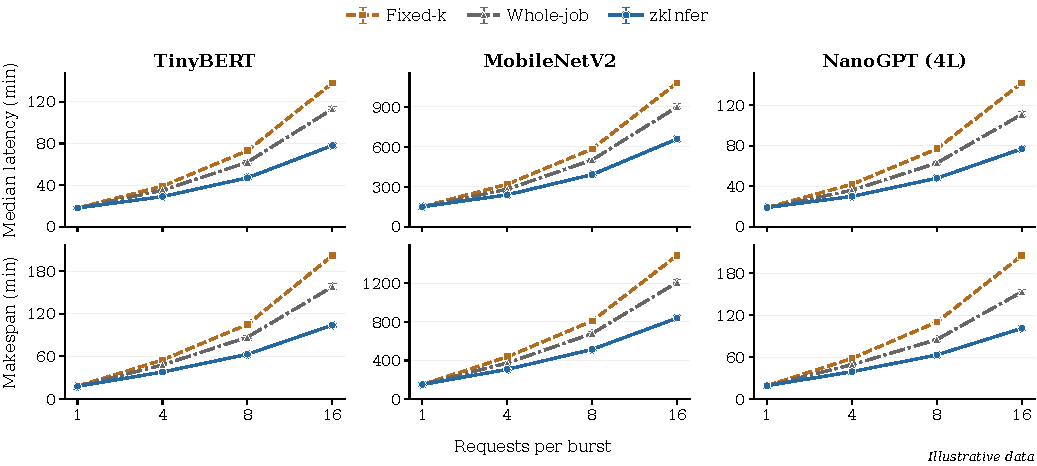
\includegraphics[width=0.95\linewidth]{figures/sacdad/eval/burst_serving.pdf}
\caption{End-to-end latency under burst arrivals on a single prover node.
We submit \(N\) inference requests simultaneously and compare fixed
concurrency, whole-job peak-memory admission, and \TITLE{}'s stage-aware
admission. Each panel shows one workload; lower is better.}
\label{fig:burst-performance}
\end{figure*}


We first examine how the three policies handle increasing
concurrent demand on a single prover node.
Figure~\ref{fig:burst-performance} reports mean request
completion time and burst makespan for each workload.


At \(N=1\), the comparison isolates concurrency among proof
jobs belonging to a single inference request.
\zkTBC{Describe the differences between policies and identify
which workloads benefit from overlapping jobs within a request.}
As \(N\) increases, jobs from multiple requests compete for
the same machine.
\zkTBC{Describe how completion time and makespan grow with
request count, including where the policies begin to diverge.}

At \(N=\zkTBC{N}\), stage-level admission changes mean request
completion time by \zkTBC{X\%} and makespan by \zkTBC{Y\%}
relative to whole-job reservation for \zkTBC{workload}.
\zkTBC{Explain whether the resource traces show additional
overlap during lower-memory stages, and report the associated
memory use and admission waiting.}
Compared with fixed concurrency, \zkTBC{describe whether
adaptive admission improves execution and where a fixed
limit remains competitive}.

The effect varies across workloads.
\zkTBC{Connect the observed differences to job heterogeneity,
stage-level memory variation, and CPU contention. Include
cases with little benefit or a regression.}
These results \zkTBC{state the supported conclusion about
stage-level admission under increasing concurrent demand}.


\subsection{Single-Request Scale-Out}
\label{sec:eval-scale-out}

We next examine how distributing proof jobs across machines affects the
completion time of an individual inference request. For each workload, we
hold the request and partitioning fixed and vary the prover pool from 1 to
10 nodes. Figure~\ref{fig:scale-out} reports request completion time and
speedup relative to one-node execution. Let \(T_p\) denote the completion
time using \(p\) prover nodes. We define speedup as \(T_1/T_p\).

All three workloads benefit substantially from additional nodes. NanoGPT
(4L) decreases from 1108~s on one node to 89~s on ten nodes, a
\(12.4\times\) speedup. MobileNetV2 decreases from 9639~s to 762~s,
yielding a \(12.7\times\) speedup, while TinyBERT decreases from 7900~s
to 750~s, a \(10.5\times\) speedup.
The scaling reflects effective distribution of the same proof workload
across additional nodes. At 10 nodes, summed job runtime per worker varies
by only 116.8--118.2~s for NanoGPT (4L) and 557.1--560.1~s for
MobileNetV2, while aggregate proving time remains nearly unchanged across
node counts. The reduction in completion time therefore comes primarily
from parallel execution rather than less proving work.

\textbf{Scale-out overhead.}
Table~\ref{tab:scaleout-overhead} breaks down aggregate job-level time
during the scale-out experiments. Proof generation remains the dominant
compute cost, averaging 746~s for NanoGPT (4L) and 4233~s for
MobileNetV2, compared with only 7~s and 32~s for verification. Shared
storage contributes mainly through reads rather than writes, with mean
aggregate S3 read times of 264~s and 820~s, while writes account for only
20~s and 18~s, respectively.
These transfer costs remain broadly stable as the prover pool grows.
Across 1--10 nodes, aggregate S3 read time ranges from 247--274~s for
NanoGPT and 798--848~s for MobileNetV2. Thus, increasing the number of
prover nodes does not substantially increase the total transfer cost for
a fixed request over the evaluated range, while proof generation remains
the dominant component.


% In the evaluation section
\begin{figure}[t]
    \centering
    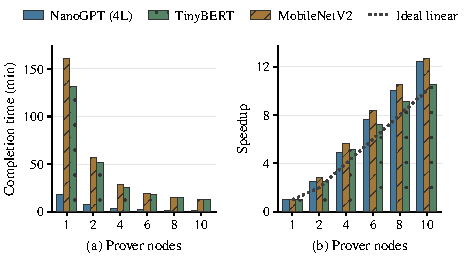
\includegraphics[width=\columnwidth]{figures/sacdad/eval/single_request_scaleout.pdf}
    \caption{
        Single-request scale-out across prover nodes.
        (a) Request completion time.
        (b) Speedup relative to one node, with ideal linear
        speedup shown as a dotted line.
        Partitioning and setup condition remain fixed.
    }
    \label{fig:scale-out}
\end{figure}

\begin{table}[t]
\centering
\small
\setlength{\tabcolsep}{3pt}
\renewcommand{\arraystretch}{1.08}
\begin{tabular*}{\columnwidth}{@{\extracolsep{\fill}}lrrrr@{}}
\toprule
& \multicolumn{2}{c}{Compute} & \multicolumn{2}{c}{Shared storage} \\
\cmidrule(lr){2-3}\cmidrule(lr){4-5}
Workload & Proving (s)   & Verify (s)  & S3 read (s) & S3 write (s) \\
         % & (s)     & (s)    & (s)     & (s) \\
\midrule
TinyBERT  & 4233.1 & 31.8 & 819.9 & 17.5 \\
MobileNetV2  & 4233.1 & 31.8 & 819.9 & 17.5 \\
NanoGPT (4L) & 746.3  & 7.1  & 264.0 & 20.3 \\


\bottomrule
\end{tabular*}
\caption{Mean aggregate job-level time across the 1--10 node
scale-out runs. Execution and transfer times are summed across proof
jobs and may overlap in wall-clock execution.}
\label{tab:scaleout-overhead}
\end{table}



% \subsection{Contribution of Resource-Management Mechanisms}
% \label{sec:eval-admission}

\subsection{Resource Profile Accuracy}
\label{sec:profile-accuracy}

\TITLE{} relies on recent executions of the same model partition to
estimate the memory required by each proving stage. We therefore evaluate
whether stage-level memory demand is sufficiently repeatable for this
history to support admission decisions. The microbenchmark repeatedly
executes representative partitions in isolation and records the peak
memory observed within each admission-relevant execution region. Cold
runs use the fused setup-and-prove region, while warm runs measure the
proving stage after reusable setup artifacts are available.

For each stage execution, we construct the prediction using only earlier
observations from the same partition and setup condition. With fewer than
five prior measurements, \TITLE{} uses the largest observed peak. Once
five observations are available, it uses the empirical 90th percentile
of the recent history. Figure~\ref{fig:profile-accuracy} reports the
median absolute prediction error and the fraction of predictions that
underestimate the subsequently observed peak.

Memory demand is highly repeatable across all three workloads. Median
absolute prediction error remains below 0.5\% in every measured
configuration. Under cold execution, the median error is 0.45\% for
MNIST GAN, 0.21\% for MobileNetV2, and 0.29\% for NanoGPT (4L). Warm
execution further reduces the error to 0.36\%, 0.15\%, and 0.07\%,
respectively. Some predictions still underestimate the observed peak, but the frequency
of these events should be interpreted together with their magnitude.
Underestimation occurs in 12.5--29.2\% of the measured cases, depending
on workload and setup condition. However, the resulting shortfalls are
small in the measurements available for these workloads, with the largest
observed shortfall remaining below 0.08~GiB. Thus, an underestimate
typically reflects a small deviation around an otherwise stable memory
profile rather than a large miss in required capacity.

\begin{figure}[t]
    \centering
    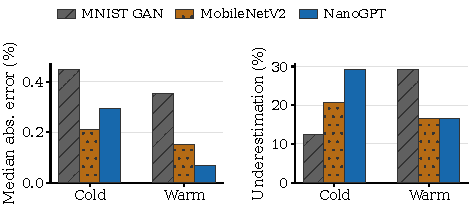
\includegraphics[width=\columnwidth]{figures/sacdad/eval/profile_accuracy_conditions.pdf}
    \caption{
    Accuracy of stage-level memory prediction under cold and warm
    execution. The left panel reports median absolute prediction error,
    while the right panel reports the fraction of predictions that
    underestimate observed memory demand. Predictions use only
    measurements from prior executions of the same partition and setup
    condition.
    }
    \label{fig:profile-accuracy}
\end{figure}

\subsection{Setup Reuse and Partition Granularity}
\label{sec:eval-sensitivity}

\textbf{Setup reuse.}
Table~\ref{tab:setup-reuse} compares the cost of generating
circuit-specific setup artifacts with reusing artifacts already available
in the node-local cache. Reuse reduces setup time by 98.6\% for TinyBERT,
97.3\% for MobileNetV2, and 96.3\% for NanoGPT (4L). In absolute terms,
MobileNetV2 falls from 14{,}609~s to 391~s, while TinyBERT and NanoGPT
fall from 1{,}636~s to 24~s and from 1{,}812~s to 67~s, respectively.
These reductions come with a sizeable storage footprint. The corresponding
proving keys occupy 68.8~GiB for TinyBERT, 287.5~GiB for MobileNetV2,
and 59.1~GiB for NanoGPT (4L). Reusing setup therefore removes most of
the repeated setup cost, but retaining every artifact locally is not
practical. This motivates the bounded per-node cache used by \TITLE{}.

\begin{table}[t]
\centering
\small
\setlength{\tabcolsep}{2.5pt}
\renewcommand{\arraystretch}{1.08}
\begin{tabular*}{\columnwidth}{@{\extracolsep{\fill}}lrrrr@{}}
\toprule
Workload & Gen. (s) & Reuse (s) & Saving (\%) & PK (GiB) \\
\midrule
TinyBERT      & 1{,}636.3  & 23.5  & 98.6 & 68.8 \\
MobileNetV2   & 14{,}608.7 & 391.0 & 97.3 & 287.5 \\
NanoGPT (4L)  & 1{,}812.3  & 67.1  & 96.3 & 59.1 \\
\bottomrule
\end{tabular*}
\caption{Cost of generating and reusing setup artifacts.}
\label{tab:setup-reuse}
\end{table}

\begin{figure}[t]
    \centering
    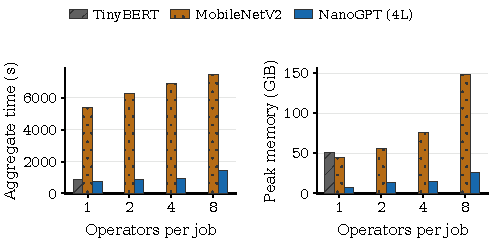
\includegraphics[width=\columnwidth]{figures/sacdad/eval/partition_granularity.pdf}
    \caption{
        Effect of partition granularity on proving cost and memory demand.
        Increasing the number of operators per proof job increases aggregate
        prover time and the peak memory required by individual jobs.
        }
\label{fig:partition-granularity}
    \label{fig:partition-granularity}
\end{figure}


\textbf{Partition granularity.}
We vary the number of operators grouped into each proof job while holding
the model and proving backend fixed. Figure~\ref{fig:partition-granularity}
shows that coarser partitions increase both aggregate prover time and peak
job memory, while exposing fewer independently schedulable jobs. We
therefore use one operator per proof job in the main serving experiments,
which provides the finest scheduling granularity and the lowest resource
demand among the configurations evaluated.


% \subsection{Contribution of Resource-Management Mechanisms}
% \label{sec:eval-admission}

% \paragraph{Memory reservation granularity.}
% To isolate admission, we compare whole-job and stage reservations while retaining
% the same coordinator policy, artifact state, and profile history. We repeat the
% eight- and sixteen-request experiments under 64, 128, and 256~GiB budgets.
% Figure~\ref{fig:eval-memory} reports the sixteen-request results. Each selected
% budget must accommodate the largest eligible job; an infeasible configuration is
% marked as such rather than treated as a completed run.

% \begin{figure*}[t]
% \centering
% \evalplot{figures/evaluation/memory_budget.pdf}{Two rows (cold, warm) by three
% workloads. Horizontal axis: usable memory budget (64, 128, 256 GiB).
% Vertical axis: batch makespan (minutes). Two curves: Whole-job and zkInfer.
% Sixteen requests per trial.}
% \caption{Effect of memory budget and reservation granularity on batch makespan.
% CPU capacity and coordinator policy remain fixed. Cold and warm executions use
% separate, matching histories. Error bars show the range across repeated trials.}
% \label{fig:eval-memory}
% \end{figure*}

% We compare the timing results with actual memory consumption and admission waits.
% A representative execution trace shows which stages overlap and whether the
% node remains memory-limited or instead reaches a CPU or storage bottleneck.
% Whole-job reservations cover the prover pipeline and output publication;
% supervisor-side artifact materialization precedes that reservation in the current
% implementation. The same boundary is used in every whole-job run. Keeping the
% selection policy fixed does not imply identical job order, since admission can
% change when jobs become runnable.
% \evalpending{Quantify improvements or regressions, peak actual memory, failures,
% and the cold/warm difference. Relate measured overlap to the motivation's packing
% opportunity without equating simulated makespan with real performance.}

% \paragraph{Coordinator scheduling.}
% We then keep stage admission enabled and compare request-fair FIFO, longest
% predicted job first within the selected request (LPT), and zkInfer's
% resource-aware coordinator policy. FIFO and LPT use the same current-free-memory
% feasibility check, so their comparison isolates within-request ordering more
% directly. The resource-aware policy additionally changes feasibility checking
% and uses cached setup and predicted duration as placement preferences. Its
% comparison is therefore a coordinator-policy ablation, not an isolated test of
% cache locality or LPT. Request fairness remains enabled in all three policies.

% \begin{table}[t]
% \centering\small\setlength{\tabcolsep}{3pt}
% \begin{tabular}{llrrr}
% \toprule
% Model & Policy & \shortstack{Median\\(min)} & \shortstack{Maximum\\(min)} & \shortstack{Failed\\requests}\\
% \midrule
% MNIST GAN & FIFO & \evalna & \evalna & \evalna\\
% & LPT & \evalna & \evalna & \evalna\\
% & zkInfer & \evalna & \evalna & \evalna\\
% MobileNetV2 & FIFO & \evalna & \evalna & \evalna\\
% & LPT & \evalna & \evalna & \evalna\\
% & zkInfer & \evalna & \evalna & \evalna\\
% NanoGPT & FIFO & \evalna & \evalna & \evalna\\
% & LPT & \evalna & \evalna & \evalna\\
% & zkInfer & \evalna & \evalna & \evalna\\
% \bottomrule
% \end{tabular}
% \caption{Coordinator-policy ablation with stage admission, warm setup,
% 16 requests, and a 256~GiB budget. Latency columns report means of per-trial
% statistics; failed requests are counted across trials. Dashes are pending.}
% \label{tab:eval-scheduling}
% \end{table}

% Table~\ref{tab:eval-scheduling} reports the resulting request latencies. For the
% mixed workload, we additionally normalize each request's latency by its model's
% isolated latency under the same setup condition. This avoids treating a naturally
% longer model as unfairly delayed solely because its absolute latency is larger.
% \evalpending{Explain which scheduling choices affect request completion and
% whether the benefit is consistent across models; report per-model slowdown for
% the mixture. A pure locality or fairness-off claim needs a separate toggle.}

% \paragraph{Setup reuse.}
% \label{sec:eval-reuse}

% The characterization established the aggregate setup time and storage associated
% with reusable artifacts. Here we measure the effect on complete requests,
% including queueing and concurrent execution. We compare cold and warm zkInfer
% runs for one and eight requests, holding partitioning, hardware, admission, and
% coordinator policy fixed. Each condition uses matching historical profiles.
% Cold runs regenerate setup; warm runs load matching artifacts from local files.

% \begin{table}[t]
% \centering\small\setlength{\tabcolsep}{3pt}
% \begin{tabular}{lrrrr}
% \toprule
% & \multicolumn{2}{c}{One request (min)} & \multicolumn{2}{c}{Eight requests (min)}\\
% \cmidrule(lr){2-3}\cmidrule(lr){4-5}
% Model & Cold & Warm & Cold & Warm\\
% \midrule
% MNIST GAN & \evalna & \evalna & \evalna & \evalna\\
% MobileNetV2 & \evalna & \evalna & \evalna & \evalna\\
% NanoGPT (4L) & \evalna & \evalna & \evalna & \evalna\\
% \bottomrule
% \end{tabular}
% \caption{Effect of setup reuse on completion time. One-request columns report
% request latency; eight-request columns report batch makespan. Entries are trial
% means; dashes mark pending measurements.}
% \label{tab:eval-reuse}
% \end{table} Table~\ref{tab:eval-reuse} connects avoided setup work to request-level benefit.
% Warm execution also changes which stages consume time and memory, so its effect
% on concurrency need not equal the reduction in summed setup time. We interpret
% the completion-time results together with setup-hit counts and measured loading
% costs. \evalpending{Report the observed latency/makespan reductions and explain
% any departure from the aggregate setup-time savings. Do not interpret these
% local-reuse measurements as a quantified remote-retrieval or locality benefit.}






% \subsection{Impact of Partition Granularity}
% \label{sec:eval-granularity}

% Partition granularity determines both the cost of individual
% proof jobs and the number of jobs available for concurrent
% execution. Combining more operators into each partition
% reduces the number of jobs, but may increase their execution
% time and memory requirements. We evaluate how this trade-off
% affects zkInfer's end-to-end performance.

% \textbf{Method.}
% For each of the three primary workloads, we vary the maximum
% number of operators per partition over
% $g \in \{1,2,4,8\}$. Operators are grouped consecutively in
% topological order, with $g=1$ corresponding to the default
% operator-level partitioning. All configurations use zkInfer's
% stage-based admission, the same prover thread settings, and
% a 256~GiB proof-memory budget on the single-node platform.
% We collect separate resource profiles and generate matching
% setup artifacts for each partitioning configuration.

% We evaluate a single inference request and a fixed batch of
% sixteen simultaneously submitted requests. The single-request
% experiment measures how granularity affects the completion
% of one inference, while the batch experiment examines how
% the resulting jobs share resources across requests.
% We report single-request latency and batch makespan across
% three trials per configuration. The $g=1$ results are reused
% from Section~\ref{sec:eval-serving}.

% \begin{figure*}[t]
% \centering
% \evalplot{figures/evaluation/partition_granularity.pdf}{
% Two rows by three workload columns: MNIST GAN,
% MobileNetV2, and NanoGPT (4L).
% Horizontal axis: maximum operators per partition,
% $g \in \{1,2,4,8\}$.
% Top row: single-request latency (minutes).
% Bottom row: sixteen-request batch makespan (minutes).
% One curve per panel: zkInfer.
% Points show the median across three trials;
% error bars show the observed minimum and maximum.
% }
% \caption{Sensitivity of zkInfer to partition granularity
% under a 256~GiB proof-memory budget.
% Each column corresponds to one workload.
% Setup artifacts are reused, and each partitioning
% configuration uses matching resource profiles.
% Lower completion times are better.}
% \label{fig:eval-granularity}
% \end{figure*}

% \textbf{Single-request performance.}
% Figure~\ref{fig:eval-granularity} shows how request latency
% changes as more operators are assigned to each proof job.
% \evalpending{Report the latency at each granularity, identify
% the best observed configuration for each workload, and
% quantify the difference relative to $g=1$. State whether
% the trend is monotonic or whether an intermediate
% granularity performs best.}

% To interpret these results, we examine the isolated job
% profiles collected for each configuration. Aggregate job
% duration captures changes in total execution work, while
% the longest job and largest memory footprint indicate
% potential limits on concurrent execution.
% \evalpending{Connect the observed latency changes to measured
% changes in these quantities and to runtime admission waiting.
% Do not attribute an improvement to lower scheduling or
% communication overhead unless the corresponding measurements
% support that explanation.}

% \textbf{Concurrent-request performance.}
% The sixteen-request experiment holds the total number of
% inferences fixed while changing the proof jobs generated
% by each request.
% \evalpending{Report batch makespan across granularities and
% the change relative to $g=1$. Explain whether the preferred
% granularity matches the single-request result, and whether
% the performance differences become larger or smaller under
% concurrent requests.}

% Multiple requests provide additional independent jobs that
% may compensate for the reduced job count of a coarser
% partitioning. However, larger per-job memory requirements
% can still restrict how many jobs execute together.
% \evalpending{Use measured memory demand, admission waiting,
% and worker utilization to explain which effect is visible
% in the results. If the measurements do not distinguish the
% causes, describe the observed trend without assigning one.}

% \textbf{Implication.}
% \evalpending{State whether the default $g=1$ configuration
% performs best, remains close to the best observed result,
% or incurs a meaningful penalty. Quantify that conclusion
% and identify any workload-dependent exceptions. If a coarser
% configuration performs better, distinguish the default's
% simplicity from its measured performance rather than
% claiming that operator-level partitioning is optimal.}


\section{Related Work}
\label{sec:related-work}

\noindent\textbf{zkML systems and prover optimization.}
Prior zkML systems reduce proving cost through specialized representations,
protocols, and compilation techniques. ZEN~\cite{boyuan2021zen},
Mystique~\cite{weng2021mystique}, and zkCNN~\cite{liu2021zkcnn} optimize
neural-network proving, while newer systems such as
ZKML~\cite{chen2024zkml}, zkLLM~\cite{sin2024zkllm}, and
ZKPyTorch~\cite{xie2025zkpytorch} extend support to broader workloads.
\TITLE{} is complementary: it leaves the proving protocol unchanged and
focuses on executing the resulting proof work under concurrent requests.

\noindent\textbf{Partitioning and distributed proving.}
DIZK~\cite{wu2018dizk} and Pianist~\cite{liu2024pianist} distribute proof
generation across machines to scale beyond a single prover. Within zkML,
ZKTorch~\cite{chen2025zktorch} exposes parallelism through specialized
basic blocks and parallel proof accumulation, while
DSperse~\cite{ivanov2025dsperse} considers proofs over selected model
slices. Recent orchestration work such as push0~\cite{ahmadvand2026push0}
addresses dispatch and recovery for distributed blockchain proving. These
systems primarily scale an individual proof computation or proving pipeline.
\TITLE{} instead treats proof jobs from concurrent inference requests as a
shared serving workload with scheduling and resource management across the
prover pool.

\noindent\textbf{ML serving systems.}
Clipper~\cite{crankshaw2017clipper}, Clockwork~\cite{gujarati2020serving},
INFaaS~\cite{romero2021infaas}, and Ray Serve~\cite{rayserve} manage
concurrent inference workloads across shared resources. zkML serving differs
in that one request may expand into long-running proof jobs with
stage-varying memory demand and reusable proving artifacts. \TITLE{} applies
serving principles to these proof-specific constraints through request-level
placement and node-local admission.

\section{Discussion}
\label{sec:discussion}
\TITLE{} uses memory as the primary admission resource because memory capacity
determines whether proof stages can safely overlap on a node. The same
framework could incorporate CPU estimates when CPU contention dominates. We
also treat partitioning and runtime scheduling separately: partitioning defines
the proof jobs, while \TITLE{} controls their execution. Finally, the
coordinator provides request-level fairness rather than explicit deadlines or
priorities, which could be added as alternative scheduling objectives.

\section{Conclusion}
\TITLE{} treats partitioned zkML proof generation as a distributed serving
problem. It separates cluster-wide job placement from node-local stage
admission, uses historical resource profiles to control memory safely, and
reuses expensive setup artifacts across requests. Our evaluation shows that
partitioning exposes heterogeneous proof jobs with strongly time-varying memory
demand and that those jobs scale effectively across prover nodes.
\textbf{[Insert final concurrent-serving headline result.]}


% ---------------------------------------------------------------------
% Bibliography
% ---------------------------------------------------------------------
\printbibliography



\end{document}